\subsection{MIR Module Entities}

\begin{figure}
  \centering
  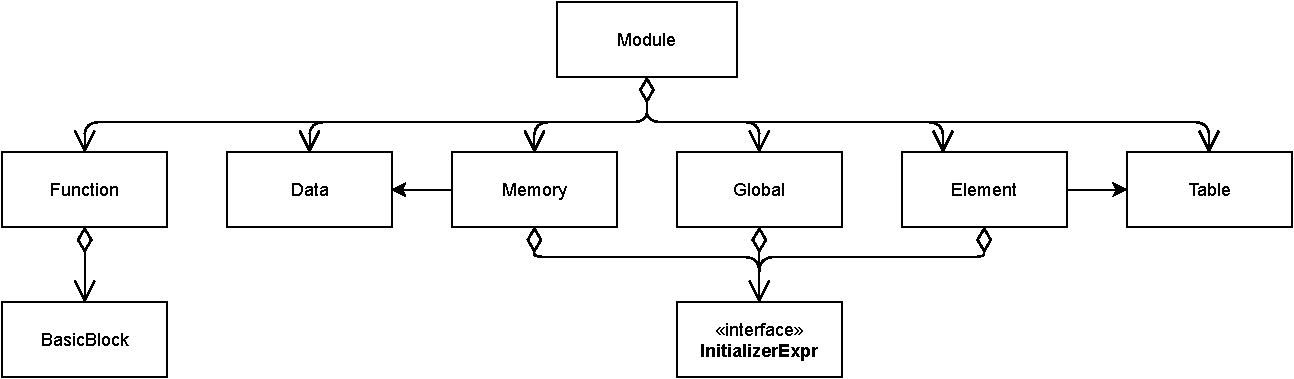
\includegraphics[width=\textwidth]{Images/4.MIR/module.pdf}
  \caption{SableWasm MIR Module-level entities}
  \label{fig:sablewasm-mir-module}
\end{figure}

SableWasm module-level entities are the top-level elements in a translation module. They are direct implements of the WebAssembly module entities defined in the specification. Figure~\ref{fig:sablewasm-mir-module} presents a general illustration of the SableWasm module-level entities. In this section, we will cover the design of each entity and compare them with its WebAssembly correspondent.

\paragraph{Function}
In figure~\ref{fig:mir-fibonacci}, we have a function definition at line 8. A function declaration in SableWasm provides information about the type, local variables and name. A function definition should satisfy all the requirements of function declaration, and additionally, provides a function body using basic blocks. The design of the function declaration and definition in SableWasm is quite similar to that of WebAssembly. The major difference is how to represent the function body. We will come back to this in the later sections within the chapter. Finally, like other module-level entities, a SableWasm function can optionally have import or export annotations. These annotations provide names for the import and export entries in the WebAssembly module.

\paragraph{Global}
SableWasm's global variable declaration and definition follow the design in WebAssembly. In SableWasm, we relax several of the constrain defined in WebAssembly specification and its extensions. In the SIMD extension proposal, the 128-bit vector type is only suitable within the function body. There is no direct way to pass a vector value to the host environment, as there is a lack of standard representation for 128-bit packed vectors in JavaScript \footnote{This might subject to change in the future. WebAssembly SIMD extension proposal is still in the drafting process.}. In  SableWasm, we treat all primitive types uniformly. Thus, a global variable can contain an integral value, a floating-point value or even a packed SIMD vector. The type for the global variable follows the specification in WebAssembly; it is a pair of value type and constness modifier. In figure~\ref{fig:mir-fibonacci}, we have a global definition at line 6, which contains a mutable 32-bit integral value. All global variable definitions in SableWasm must provide a value initialization via initializer expression, which we covered in the previous section. The rules for import and export annotation on the SableWasm function entities also apply to SableWasm global variables, which we do not show in the example above.

\paragraph{Memory and Data}
Memory and Data are implementation for WebAssembly linear memory and its initializer, respectively. One might think that there is no need to separate the memory initializer from the memory entity definition, as in WebAssembly specification, all data section entries must provide a valid linear memory index. In the early version of SableWasm, we indeed adopt such implementation. However, this approach might be subject to a significant change in an extension that might soon merge to the WebAssembly specification. The WebAssembly bulk memory operation extension proposal \footnote{WebAssembly bulk memory operations: \\\url{https://github.com/WebAssembly/bulk-memory-operations}} introduce new instructions, such as \texttt{memory.fill} that direct refers to a data section segment. Moreover, the proposal relaxes the constrain on the linear memory index. Now the index can behave like a flag indicating whether the data segment itself is active or not and no longer serves as a linear memory index. Hence, to make our framework `futureproof', we separate the linear memory declaration from their initializers. Figure~\ref{fig:mir-fibonacci} presents a linear memory definition at line 2. SableWasm memory entities also adopt WebAssembly linear memory type. The type consists of a pair of unsigned integers, indicating the lower bound and upper bound of the memory size in WebAssembly pages. Finally, the memory entity can have import and export annotations similar to other module-level entities in SableWasm. The example above defines a memory with a minimal size of 2 pages, 128KiB, and exports it under `memory'. The example above does not provide any example for data initializers, but they are quite easy to understand. A data initializer is essentially a binary chunk with an initialization offset. They are semantically equivalent to a data section entry in an ELF file.

\paragraph{Table and Element} SableWasm table and element entity implements the indirect table and its initializer, namely element segment, accordingly. They follow the simple principle as the memory and data entity in the previous section. Currently, like data segment entry, WebAssembly's element section entry must refer to a valid indirect table via an index. In the future, this may also subject to change. WebAssembly reference types extension proposal \footnote{WebAssembly reference types: \url{https://github.com/WebAssembly/reference-types}} introduce instructions such as \texttt{table.fill} that are able to have direct access to element segment initializers. \texttt{table.fill} instruction is similar to \texttt{memory.fill} defined in the bulk memory operation extension. It will copy a sequence of compile-time defined function pointers into an indirect table at runtime. Thus, when we design our table entity, we also split the declarations from their initializers. The type for table entity is the same as the table type in WebAssembly. It consists of a pair of unsigned integers, indicating the lower bound and upper bound for the number of function pointers stored in the indirect table. In SabelWasm MIR, we treat memory entities and table entities as black boxes, and its concrete implementation is deferred to the backend. The example shown in figure~\ref{fig:mir-fibonacci}, the module defines a table entity at line 4 that stores exactly one function pointers. Note that the table entity does not require users to initialize the value for all entries. The table entity default initializes all entries to null pointers. Finally, the rule for import and export annotation also apply for table entity. However, the element entity is local to the module and can neither export nor import from other modules.

In this section, we cover the design for module-level entities in SableWasm. They are pretty similar to the sections defined in WebAssembly specification. In the next section, we will move the design of SableWasm instructions.